\subsection{Resultate \label{subsec:cmb:results}}

Die Resultate 

\begin{figure}
	\centering
	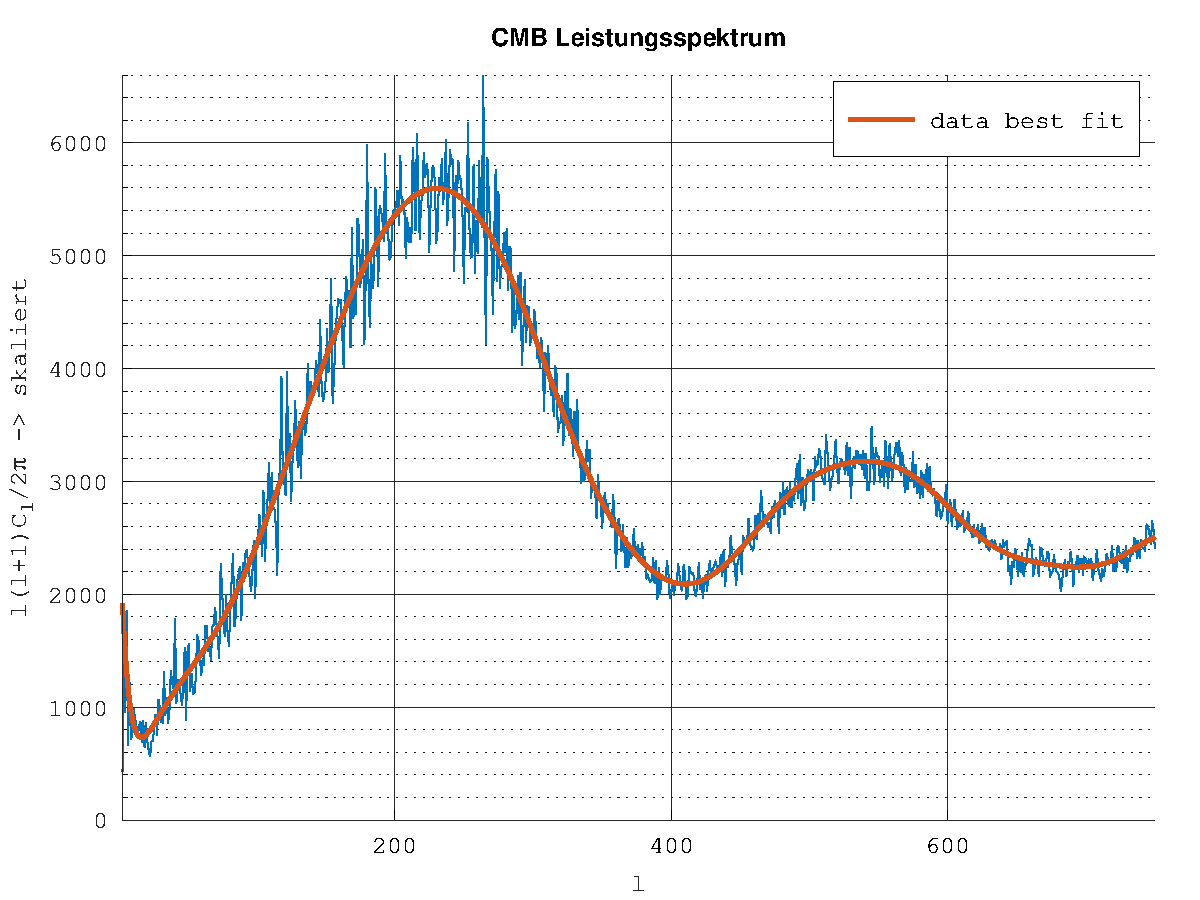
\includegraphics[width=\linewidth]{cmb/data/2k900-500.pdf}
	\caption{Leistungsspektrum berechnet bis zu $l = 900$. Grundlage für die 
		Berechnung ist das 2K aufgelöste Bild der ESA Planck Mission.}
	\label{fig:cmb-power-spec-900}
\end{figure}

\begin{figure}
	\centering
	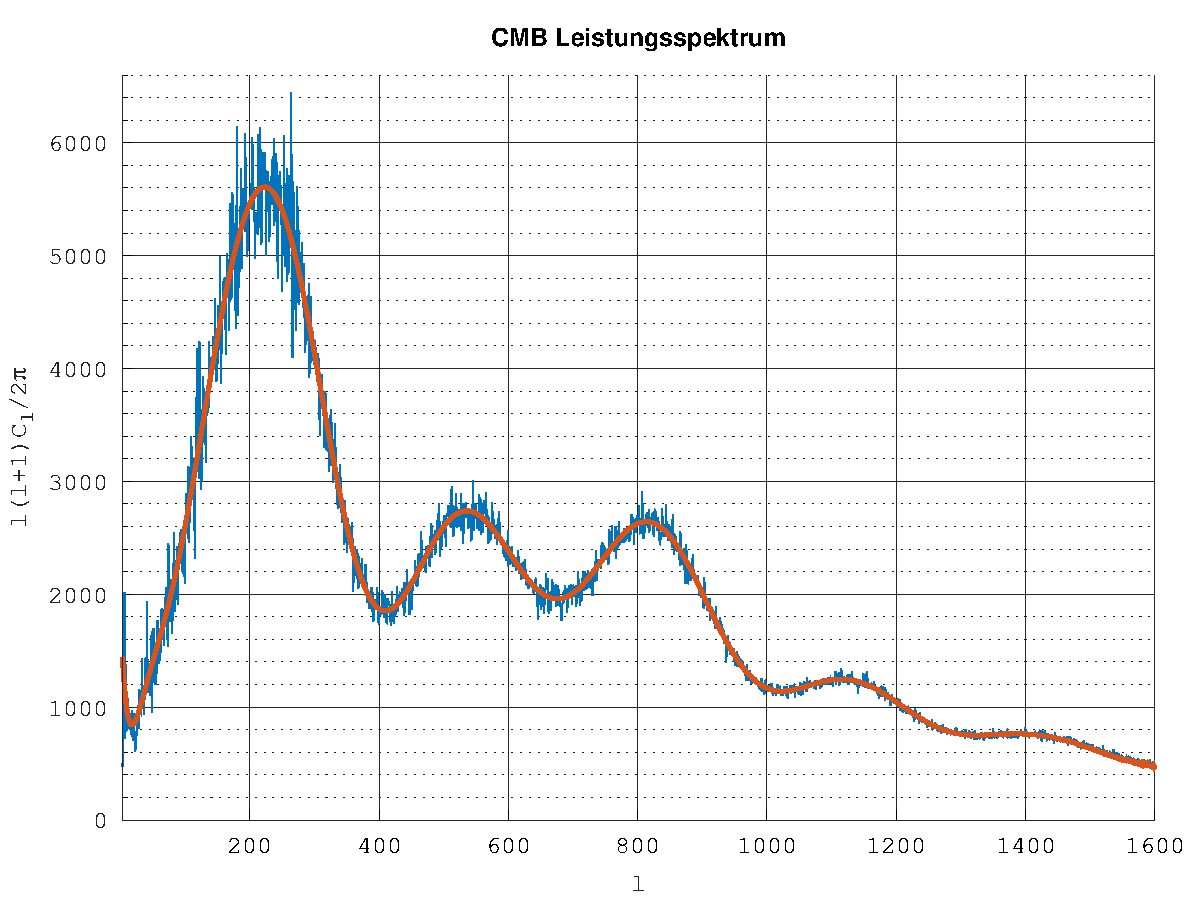
\includegraphics[width=\linewidth]{cmb/data/4k1800-500.pdf}
	\caption{Leistungsspektrum berechnet bis zu $l = 1600$. Grundlage für die 
		Berechnung ist das 4K aufgelöste Bild der ESA Planck Mission.}
	\label{fig:cmb-power-spec-1600}
\end{figure}

\begin{figure}
	\centering
	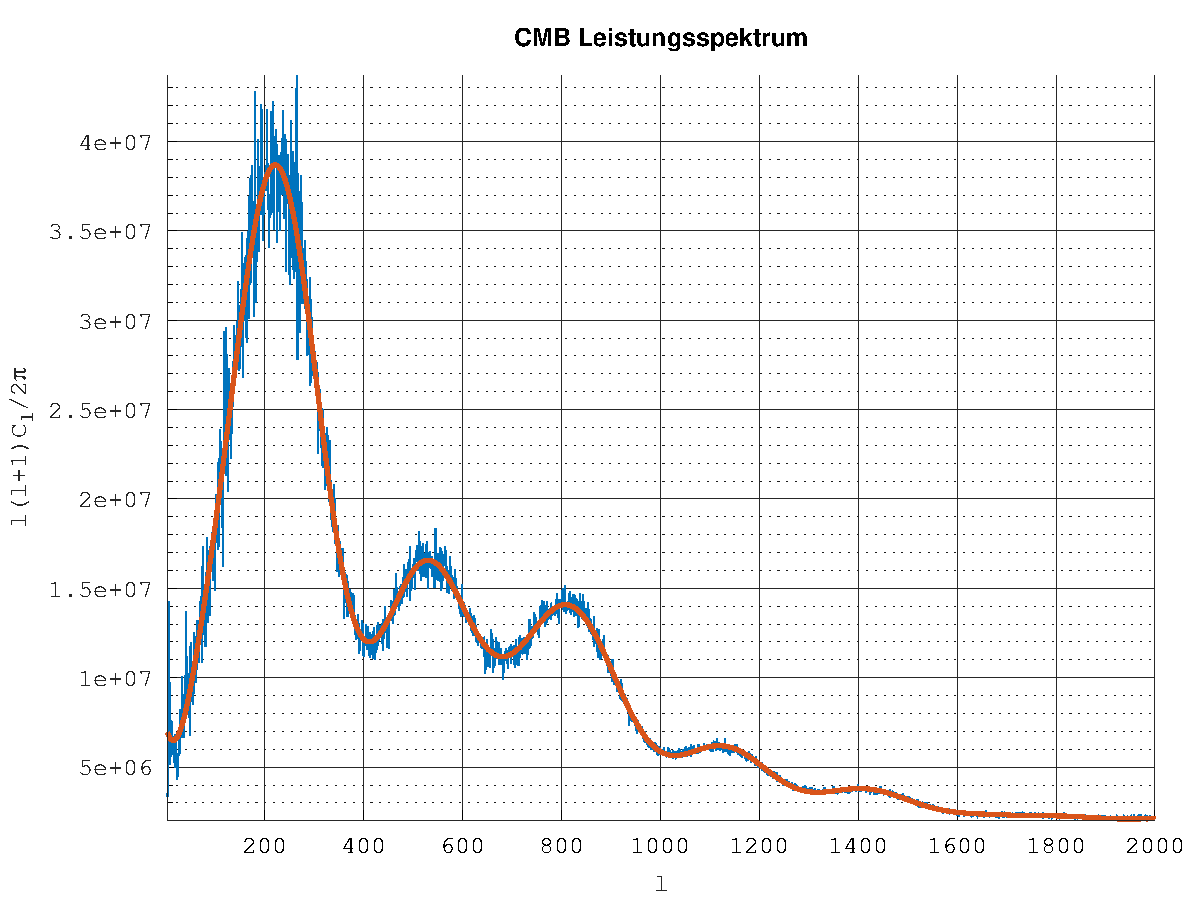
\includegraphics[width=\linewidth]{cmb/data/12k2500-500.pdf}
	\caption{Leistungsspektrum berechnet bis zu $l = 2000$. Grundlage für die 
	Berechnung ist das 12K aufgelöste Bild der ESA Planck Mission.}
	\label{fig:cmb-power-spec-2000}
\end{figure}
